\documentclass[hidelinks,12pt]{article}
\usepackage{algorithm2e}
\usepackage[brazil]{babel}
\usepackage[utf8]{inputenc}
\usepackage{listings}
\usepackage{amsmath}
\usepackage{amsfonts}
\usepackage{amssymb}
\usepackage{indentfirst}
\usepackage{caption}
\usepackage{color}
\usepackage{mathrsfs}
\usepackage{pgfplots}
\usepackage{hyperref}
\usepackage{fancyhdr}
\usepackage{verbatimbox}
\usepackage[export]{adjustbox}
\usepackage{xcolor}
\usepackage{textcomp}
\newcommand{\icon}[1]{\includegraphics[height=12pt]{#1}}
\newcommand{\bigicon}[1]{\includegraphics[height=50pt]{#1}}
% -------------------------------------------------------------------- %
% Cores para formatação de código
\usepackage{color}
\definecolor{vermelho}{rgb}{0.6,0,0} % para strings
\definecolor{verde}{rgb}{0.25,0.5,0.35} % para comentários
\definecolor{roxo}{rgb}{0.5,0,0.35} % para palavras-chaves
\definecolor{azul}{rgb}{0.25,0.35,0.75} % para strings
\definecolor{cinza-claro}{gray}{0.95}
% -------------------------------------------------------------------- %

% Declaracoes em Portugues
%\algrenewcommand\algorithmiccase{\textbf{caso}}


\DeclareCaptionFont{white}{\color{white}}
\DeclareCaptionFormat{listing}{%
	\parbox{\textwidth}{\colorbox{gray}{\parbox{\textwidth}{#1#2#3}}\vskip-4pt}}
\captionsetup[lstlisting]{format=listing,labelfont=white,textfont=white}
\lstset{frame=lrb,xleftmargin=\fboxsep,xrightmargin=-\fboxsep}


\newcommand{\iconb}[1]{\includegraphics[height=20pt]{#1}}
\setcounter{secnumdepth}{5}

\fancypagestyle{plain}{%
	\fancyfoot{}%
	\fancyhead{}%
}


\begin{document}
\pagenumbering{gobble}
\pagestyle{fancy}


\lhead{\bigicon{Figures/ufu}}
\chead{{\footnotesize UNIVERSIDADE FEDERAL DE UBERLÂNDIA \\ FACULDADE DE CIÊNCIA DA COMPUTAÇÃO \\ Construção de Compiladores} \\ \scriptsize{Av. João Naves de Ávila 2121, Campus Santa Mônica} }
\rhead{\bigicon{Figures/facom}}
\lfoot{}
\cfoot{}
\rfoot{}
\vspace*{8.5cm}
\begin{figure}[!h]
	\centering
	\Huge{\bf {Reconhecimento de padrões em matrizes utilizando Redes Neurais Perceptron}}
\end{figure}

\vspace*{5cm}

\noindent\textbf{Aluno:} Eduardo Costa de Paiva \qquad \textbf{Matrícula:} 11221BCC012 \\
\textbf{Email:} \texttt{\small \url{ eduardocspv@gmail.com}}\\
\textbf{Profº.:} Gina Maira Barbosa de Oliveira


\newpage
\fancyhead[C]{}
\fancyhead[R]{}
\fancyhead[L]{\leftmark}
\fancyfoot{}
%\fancyfoot[L]{{\footnotesize  Construção de Compiladores}}
\fancyfoot[C]{\hspace{1.5cm}\thepage}
%\fancyfoot[R]{{\footnotesize Universidade Federal de Uberlândia}}
\pagenumbering{arabic}


{\let\thefootnote\relax\footnotetext{\textit{UFU, Universidade Federal de Uberlândia, Minas Gerais, Brasil}}}

\newpage

\tableofcontents


\newpage

\section{Introdução}

	Esse relatório tem como objetivo explicar o uso das redes neurais perceptron para reconhecimento de padrões em matrizes (números 0,1,2,3,4,5). Para o primeiro exercício foi utilizado apenas 1 neurônio, para o segundo 2 neurônios e para o terceiro exercício foram utilizado 6 neurônios.
	
	O sistema operacional que utilizado foi o Ubuntu 16.04 e a para o desenvolvimento foi utilizado a linguagem {\bf{Java}}.

\section{Especificação}
		
	Os padrões foram representados por matrizes de 6 linhas e 5 colunas salvos em  arquivos \textbf{.txt}. Onde os índices marcados pelo número 1 representam o padrão desejado.
		
	\begin{figure}[h!]
		\centering
		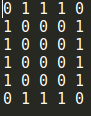
\includegraphics[scale=0.5]{Figures/number0}
		\caption{Número 0}
	\end{figure}
	
	Para o caso em que os pesos inicias são gerados aleatoriamente, estes foram gerados no intervalo de -1 a 1.
\section{Testes realizados}

\subsection{Exercício 1}
	\newpage
	\large {\textbf{Pesos inicias zerados}}
	
	\subsubsection{Pesos após término do treinamento}
		\begin{figure}[h!]
			\centering
			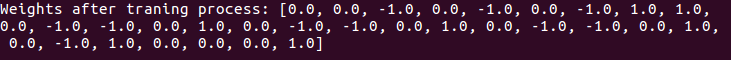
\includegraphics[scale=0.6]{Figures/pesoszeroexercicio1}
			\caption{Pesos}
		\end{figure}
		
	\subsubsection{Número de épocas e entradas distorcidas}

		\begin{figure}[h!]
			\centering
			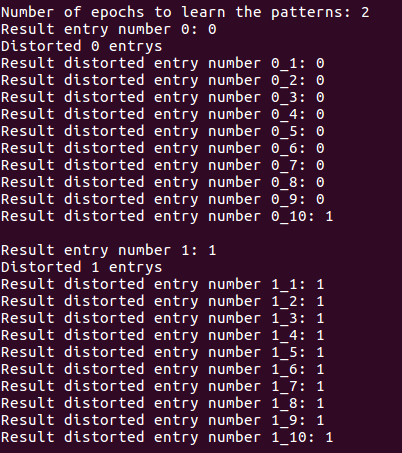
\includegraphics[scale=0.6]{Figures/epochsexercicio1}
			\caption{Número de épocas e resultados para entradas distorcidas}
		\end{figure}
		
	\newpage
	\subsubsection{Saída para as entradas 2,3,4,5 }

		\begin{figure}[h!]
			\centering
			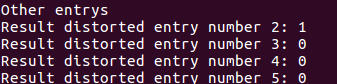
\includegraphics[scale=0.6]{Figures/outrasentradasexercicio1}
			\caption{Resultado para os padrões 2,3,4,5}
		\end{figure}
	
	{\textbf{\large Pesos inicias aleatórios}}
	
	\subsubsection{Pesos após término do treinamento iniciando-os aleatoriamente}

		\begin{figure}[h!]
			\centering
			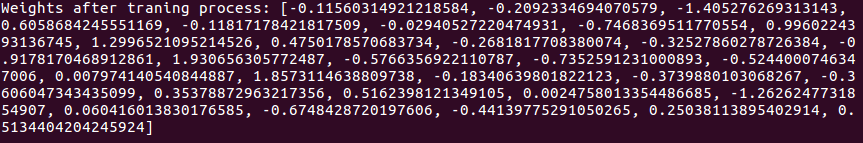
\includegraphics[scale=0.5]{Figures/pesosexercicio1}
			\caption{Pesos}
		\end{figure}
	\newpage
	\subsubsection{Número de épocas e entradas distorcidas com pesos inicias aleatórios}

		\begin{figure}[h!]
			\centering
			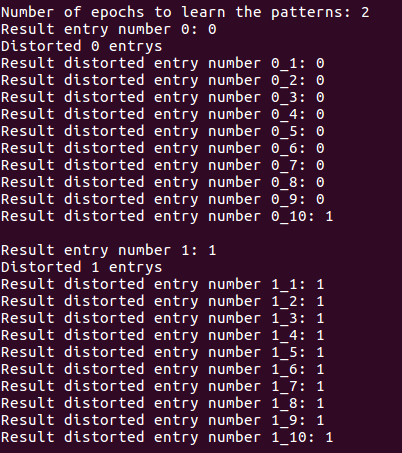
\includegraphics[scale=0.6]{Figures/epochsexercicio1}
			\caption{Número de épocas e resultados para entradas distorcidas}
		\end{figure}
	
		\normalsize Em média são gastas de 2 a 3 épocas para o treinamento.

	\newpage
	\subsubsection{Saída para as entradas 2,3,4,5}

		\begin{figure}[h!]
			\centering
			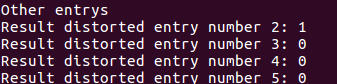
\includegraphics[scale=0.6]{Figures/outrasentradasexercicio1}
			\caption{Resultado para os padrões 2,3,4,5}
		\end{figure}

\subsection{Exercício 2}
	\large {\textbf{Pesos inicias zerados}}
	
	\subsubsection{Pesos e épocas após término do treinamento}

		\begin{figure}[h!]
			\centering
			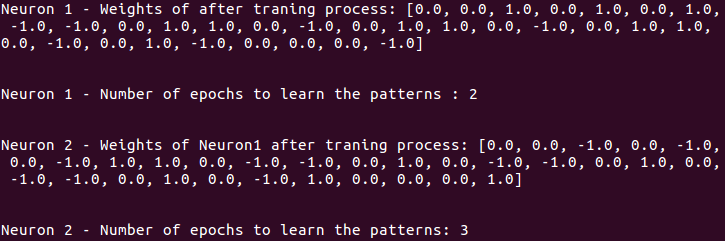
\includegraphics[scale=0.6]{Figures/epochsweightsexerc2}
			\caption{Pesos e épocas}
		\end{figure}
	\newpage
	\subsubsection{Resultados para entradas distorcidas}

		\begin{figure}[h!]
			\centering
			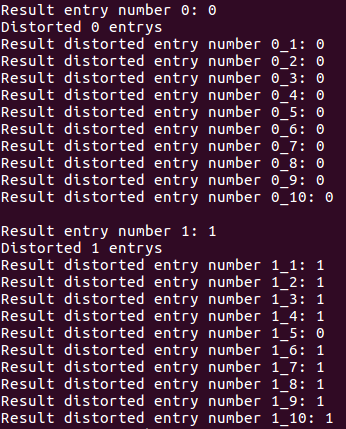
\includegraphics[scale=0.6]{Figures/distortedentrysexerc2}
			\caption{Entradas distorcidas}
		\end{figure}
		
	\subsubsection{Saída para as entradas 2,3,4,5}

		\begin{figure}[h!]
			\centering
			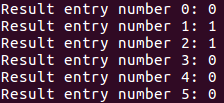
\includegraphics[scale=0.6]{Figures/otherentrysexerc2}
			\caption{Resultado para os padrões 2,3,4,5}
		\end{figure}
	
	{\textbf{\large Pesos inicias aleatórios}}
	
	\newpage
	\subsubsection{Pesos e épocas após término do treinamento com pesos inicias aleatórios}

		\begin{figure}[h!]
			\centering
			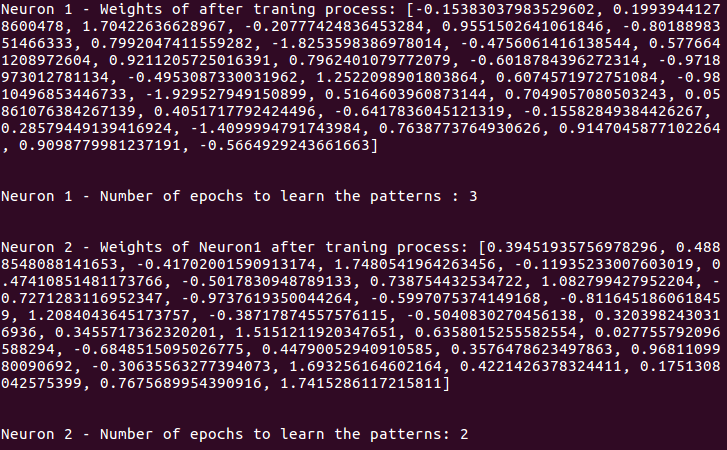
\includegraphics[scale=0.6]{Figures/epochsweightsrandomexerc2}
			\caption{Pesos e épocas}
		\end{figure}
	
		\normalsize Em média são gastas de 2 a 3 épocas para o treinamento.
	
	\subsubsection{Resultados para entradas distorcidas}

		\begin{figure}[h!]
			\centering
			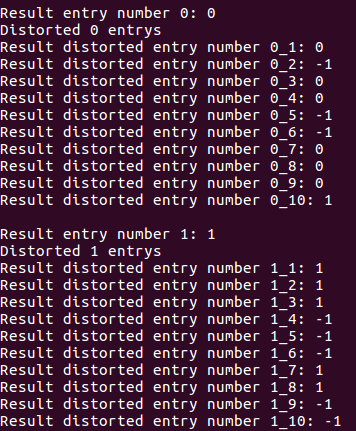
\includegraphics[scale=0.6]{Figures/distortedentrysrandomexerc2}
			\caption{Entradas distorcidas}
		\end{figure}

	\newpage
	\subsubsection{Saída para as entradas 2,3,4,5}

		\begin{figure}[h!]
			\centering
			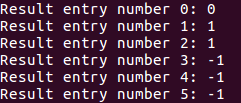
\includegraphics[scale=0.6]{Figures/otherentrysrandomexerc2}
			\caption{Resultado para os padrões 2,3,4,5}
		\end{figure}

\subsection{Exercício 3}
	\large {\textbf{Pesos inicias zerados}}
	
	\newpage
	\subsubsection{Pesos e épocas após término do treinamento}
		\begin{figure}[h!]
			\centering
			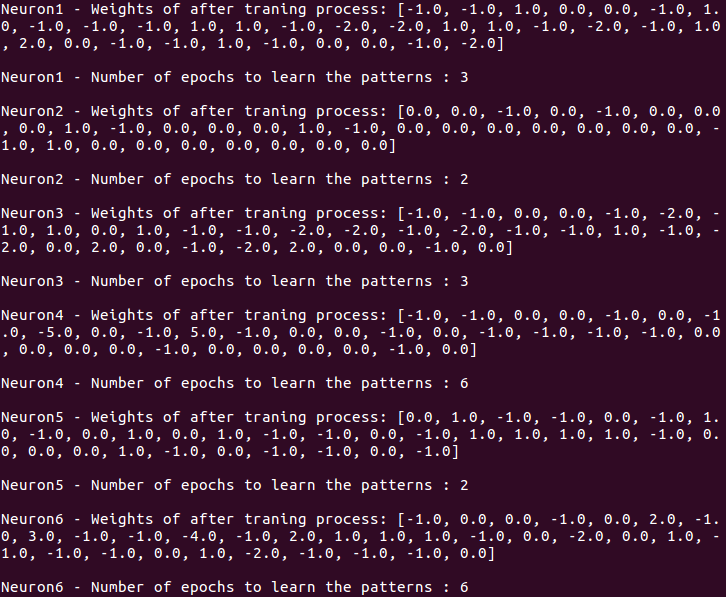
\includegraphics[scale=0.6]{Figures/epochsweightsexerc3}
			\caption{Pesos e épocas}
		\end{figure}
		
	\newpage
	\subsubsection{Resultados para entradas distorcidas}

		\begin{figure}[h!]
			\centering
			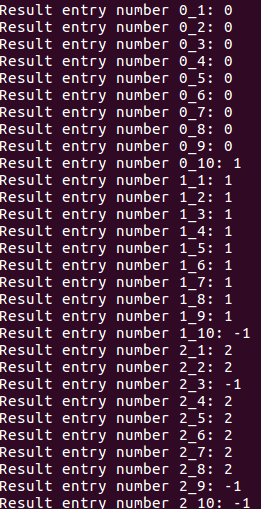
\includegraphics[scale=0.6]{Figures/distortedentrys1exerc3}
			\caption{Resultados para entradas distorcidas 0,1,2}
		\end{figure}
	
		\begin{figure}[h!]
			\centering
			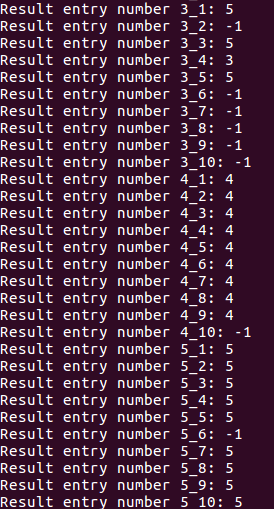
\includegraphics[scale=0.6]{Figures/distortedentrys2exerc3}
			\caption{Resultados para entradas distorcidas 3,4,5}
		\end{figure}
	\newpage
	\subsubsection{Saída para as entradas A,E,T,H,C,N}

		\begin{figure}[h!]
			\centering
			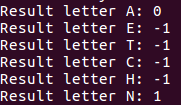
\includegraphics[scale=0.6]{Figures/lettersexerc3}
			\caption{Resultado para os padrões A,E,T,H,C,N}
		\end{figure}
	
	
	\newpage
	{\textbf{\large Pesos inicias aleatórios}}
	
	
	\subsubsection{Pesos e épocas para os neurônios 1 2 e 3, após término do treinamento com pesos inicias aleatórios}

		\begin{figure}[h!]
			\centering
			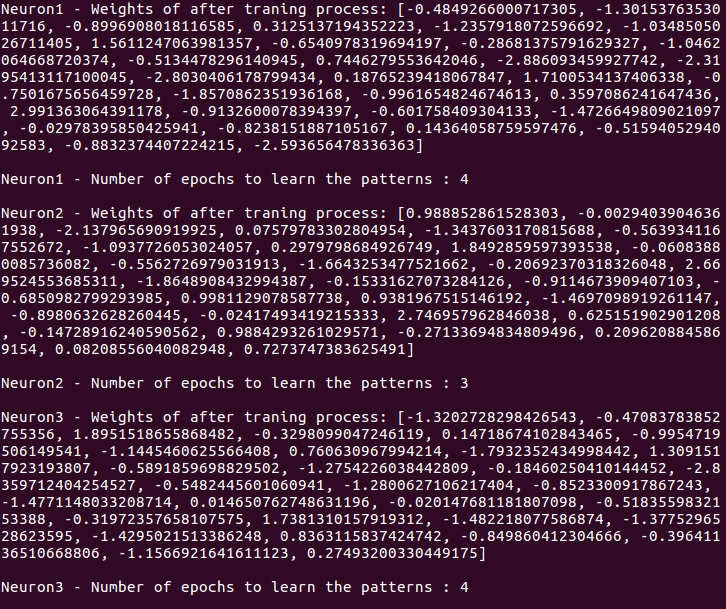
\includegraphics[scale=0.6]{Figures/epochsweightsrandom1exerc3}
			\caption{Pesos e épocas dos neurônios 1,2,3}
		\end{figure}
	
	\newpage
	\subsubsection{Pesos e épocas para os neurônios 4 5 e 6, após término do treinamento com pesos inicias aleatórios}

		\begin{figure}[h!]
			\centering
			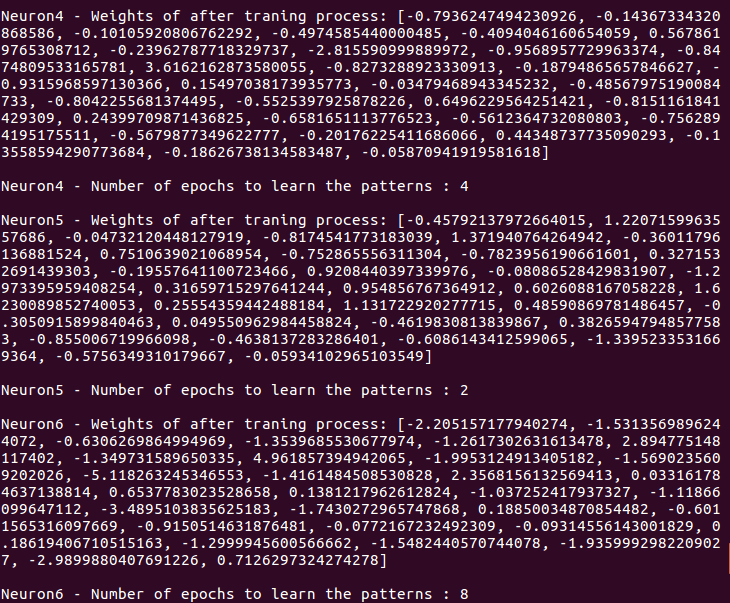
\includegraphics[scale=0.6]{Figures/epochsweightsrandom2exerc3}
			\caption{Pesos e épocas dos neurônios 4,5,6}
		\end{figure}
		
		\normalsize No treinamento, o neurônio com maior número de épocas é 8.
		
	\newpage
	\subsubsection{Resultados para entradas distorcidas}

		\begin{figure}[h!]
			\centering
			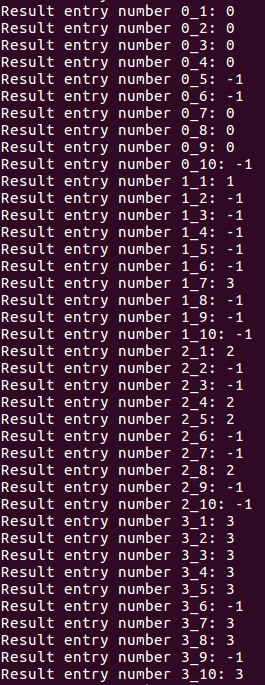
\includegraphics[scale=0.6]{Figures/distortedentrysrandom1exerc3}
			\caption{Resultados para entradas distorcidas 0,1,2,3}
		\end{figure}
		
		\begin{figure}[h!]
			\centering
			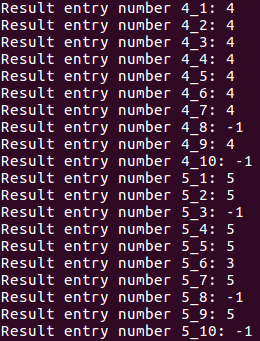
\includegraphics[scale=0.6]{Figures/distortedentrysrandom2exerc3}
			\caption{Resultados para entradas distorcidas 4 e 5}
		\end{figure}

	
		

	\newpage
	\subsubsection{Saída para as entradas A,E,T,H,C,N}

		\begin{figure}[h!]
			\centering
			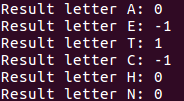
\includegraphics[scale=0.6]{Figures/lettersrandom}
			\caption{Resultado para os padrões A,E,T,H,C,N}
		\end{figure}
	
\end{document}